% !TeX spellcheck = es_ES
\chapter{Introducción}
\label{ch:chap01}

%================================================================================================
% Introducción 
%================================================================================================


%================================================================================================
% Motivación y problema
%================================================================================================

\section{Motivación y problema}
\label{sec:motivacionYProblemas}

Naturalmente, el fenómeno de la iluminación ocurre cuando una fuente luminosa emite un flujo de fotones, normalmente conocido como rayo o haz de luz, que recorre un camino hasta intersectar una superficie que lo bloquee o desvíe. Según la óptica, los fenómenos que pueden manifestarse debido a esta interacción son la \textit{absorción, reflexión, refracción}; pues una superficie puede conservar parte de la energía transmitida afectando el color percibido, reflejarla en distintas direcciones, modificar la dirección del haz al poseer propiedades de transparencia.

Para simular dicho fenómeno, se han desarrollado y formalizado un conjunto de algoritmos y herramientas que resuelven el problema con distintos niveles de complejidad y realismo físico. Para caracterizar los problemas descriptos, normalmente se utiliza un estándar conocido como expresiones de caminos de luz \cite{LPE} (o LPEs, por sus siglas en inglés). Estas expresiones regulares se establecen distintos eventos: que representados por un conjunto de letras que son leídas de izquierda a derecha, y corresponden a un camino de la luz particular. A efectos de este proyecto, interesan los objetos \textbf{C} (cámara) y \textbf{L} (emisión de luz), así como los eventos \textbf{S} (reflexión especular),  \textbf{D} (reflexión difusa).

Estas formas fundamentales son las que rigen el comportamiento de la luz cuando reflejada en la naturaleza. En la primera, la luz es reflejada en direcciones aleatorias, que idealmente son distribuidas siguiendo la distribución del coseno. Mientras que en el segundo caso, el ángulo de reflexión es igual al de incidencia como se aprecia en la Figura \ref{img:difspecularr}.

\vspace{5mm}
\begin{figure}[htbp]
	\begin{subfigure}{0.5\textwidth}
		\centering
		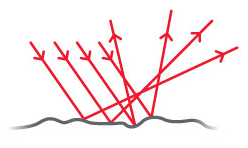
\includegraphics[width=1\linewidth]{assets/difusa1}
		\caption{Difusa}
	\end{subfigure}
	\begin{subfigure}{0.5\textwidth}
		\centering
		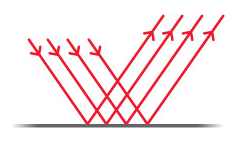
\includegraphics[width=1\linewidth]{assets/especular1}
		\caption{Especular}
	\end{subfigure}
	\caption{Posibles formas de reflexión de la luz con superficies.}
	\label{img:difspecularr}
\end{figure}

Los algoritmos de traza de rayos o radiosidad resuelven el problema de la iluminación global con distintos acercamientos. Originalmente, el algoritmo de traza de rayos contempla los caminos de luz de la forma \textbf{L{S-D}*C}, es decir, cualquier nivel de reflexiones especulares o difusas; la solución se basa en simular haces de luz (rayos) como semi-rectas, calculando los puntos de intersección con los objetos de la escena recursivamente. Por otro lado, el algoritmo de radiosidad involucra la subdivisión de una escena virtual en superficies finitas conocidas como \textit{parches} a los que se les asignará un valor de radiosidad (energía lumínica) dependiente de la ubicación de las fuentes luminosas y las oclusiones causadas por la disposición de la geometría de la escena. Esto quiere decir, que en su concepción, el algoritmo sólo considera caminos de la forma \textbf{L{D}*C}. No obstante, es deseable que los caminos especulares sean contemplados en el cálculo de la radiosidad.

Estas interacciones observadas son de gran interés para la computación gráfica, dado que su estudio tiene gran relevancia en la arquitectura y la industria del entretenimiento. En particular, la generación de modelos capaces de simular el transporte de la luz en espacios tridimensionales es uno de los mayores motivadores de los avances en computación gráfica. A lo largo de los siglos XX y XXI se han propuesto distintos modelos (\cite{Kajiya}, \cite{Cohen}) que aproximan el comportamiento real de la luz en distintos entornos con variados niveles de foto-realismo y desempeño computacional.

Si bien el trazado de rayos tiene el potencial de resolver todos los fenómenos físicos explicados anteriormente, su desempeño computacional empeora con la presencia de superficies difusas. El algoritmo de radiosidad tiene la capacidad de resolver los caminos de la forma \textbf{LD*E} (considerando únicamente el fenómeno de la reflexión difusa) de forma eficiente a través del uso de factores de vista para el modelado del fenómeno de la iluminación así como del transporte de energía térmica entre superficies.

El avance del \textit{hardware} en los últimos años obliga a revaluar los algoritmos de iluminación global constantemente, con el objetivo de proveer resultados fotorealistas en tiempos de ejecución cada vez menores. Si bien en los últimos años se han desarrollado las técnicas de \textit{trazado de rayos bi-direccional} y otras técnicas de \textit{trazado de rayos de Monte Carlo} con el objetivo de atacar el problema de la reflexión difusa utilizando el algoritmo de traza de rayos, también se han propuesto variantes que extienden los métodos de radiosidad para considerar los efectos introducidos por las superficies especulares.

%================================================================================================
% Objetivos
%================================================================================================

\section{Objetivos}
\label{sec:objetivos}

Este proyecto tiene el objetivo de analizar las técnicas de extensión del método de radiosidad a caminos de la forma \textbf{L(S$|$D)*E}, generando adaptaciones de las extensiones propuestas por trabajos previos y literatura asociada. A su vez, se generará la implementación correspondiente a los distintos algoritmos formulados con la finalidad de comparar cualitativamente el rendimiento computacional observado en hardware moderno así como el error introducido por las aproximaciones que se consideran al discretizar el problema concebido.

En este sentido, se exploran tres implementaciones diferentes para el cálculo de la radiosidad entre las superficies que componen la escena virtual considerada. Se propone aprovechar la implementación en hardware de un conjunto de funcionalidades que facilitan la proyección tridimensional así como el uso de eficiente de los recursos de cómputo a través de bibliotecas que permiten manejar el paralelismo.  

%================================================================================================
% Estructura el documento
%================================================================================================

\section{Estructura del documento}
\label{sec:estructuraDelDocumento}

El resto del documento se estructura de la siguiente manera. El Capítulo 2 introduce el estado del arte en técnicas de iluminación global, con especial énfasis en la técnica de radiosidad y sus extensiones. Además, se exploran diversos acercamientos alternativos al problema a resolver. El Capítulo 3 refiere al diseño de la solución de los algoritmos implementados. El Capítulo 4 describe la implementación realizada, detallando distintas decisiones tomadas para eludir un conjunto de obstáculos técnicos observados. En el Capítulo 5, se encuentra una síntesis de los casos de prueba considerados así como los un análisis de los resultados obtenidos junto a un conjunto de ventajas y desventajas que se han observado. Finalmente, se desarrollan las conclusiones y posible líneas de trabajo futuro detectadas a lo largo del desarrollo del proyecto.